\begin{figure}
	\center
	\begin{minipage}{0.16\linewidth}
		\center \scriptsize
		\includegraphics[width=\linewidth]{plot/oxf_cmu/Results_lt_queries/distance}	
		
		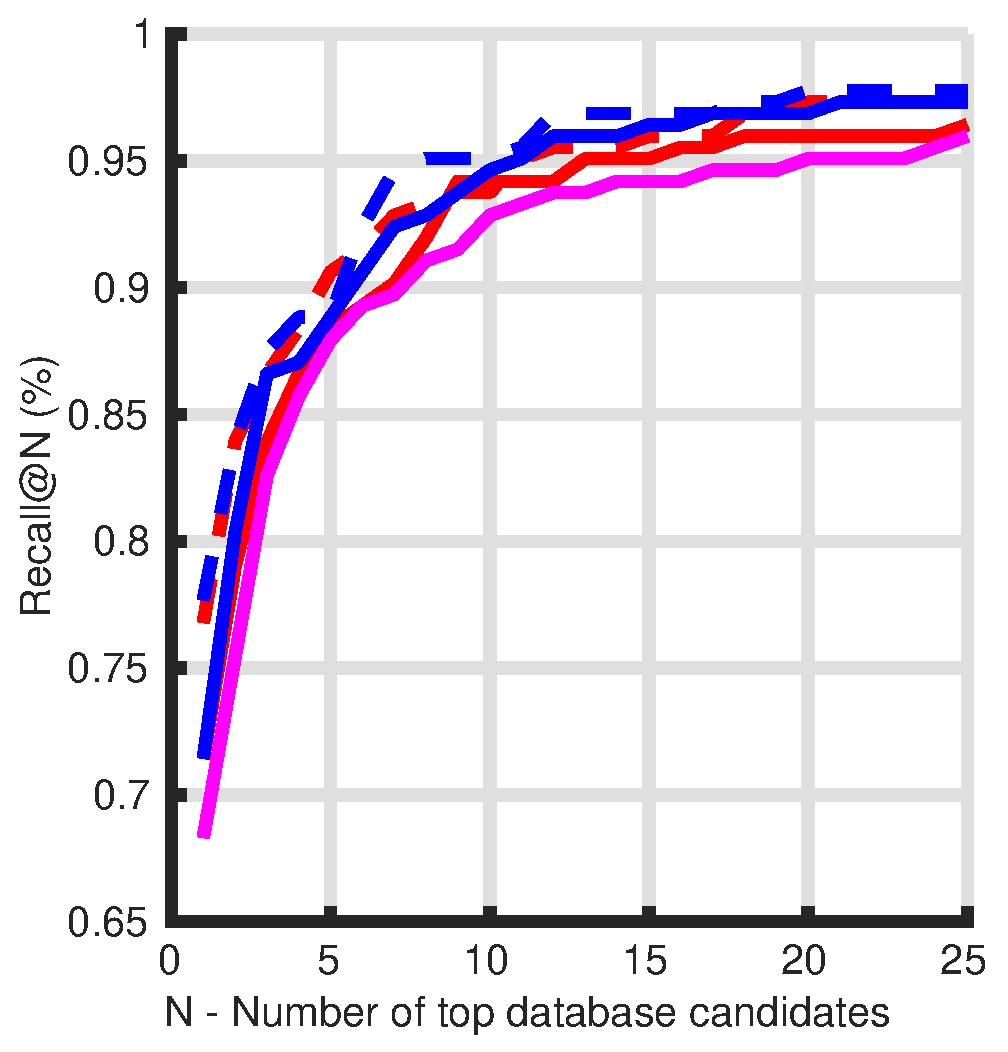
\includegraphics[width=\linewidth]{plot/oxf_cmu/Results_lt_queries/recall}
		
		a) Oxford -- LT
	\end{minipage}
	\begin{minipage}{0.16\linewidth}
		\center \scriptsize
		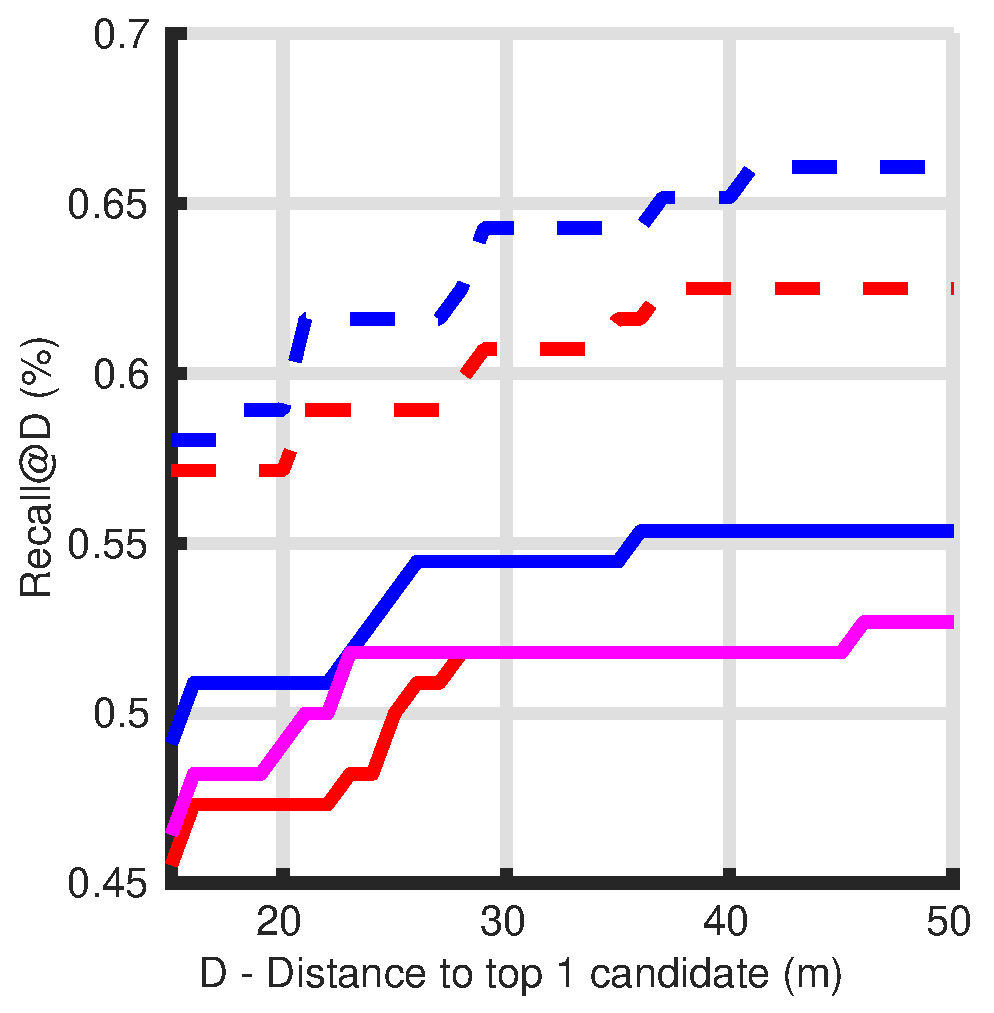
\includegraphics[width=\linewidth]{plot/oxf_cmu/Results_snow_queries/distance}	
		
		\includegraphics[width=\linewidth]{plot/oxf_cmu/Results_snow_queries/recall}
				
		b) Oxford -- Snow
	\end{minipage}
	\begin{minipage}{0.16\linewidth}
		\center \scriptsize
		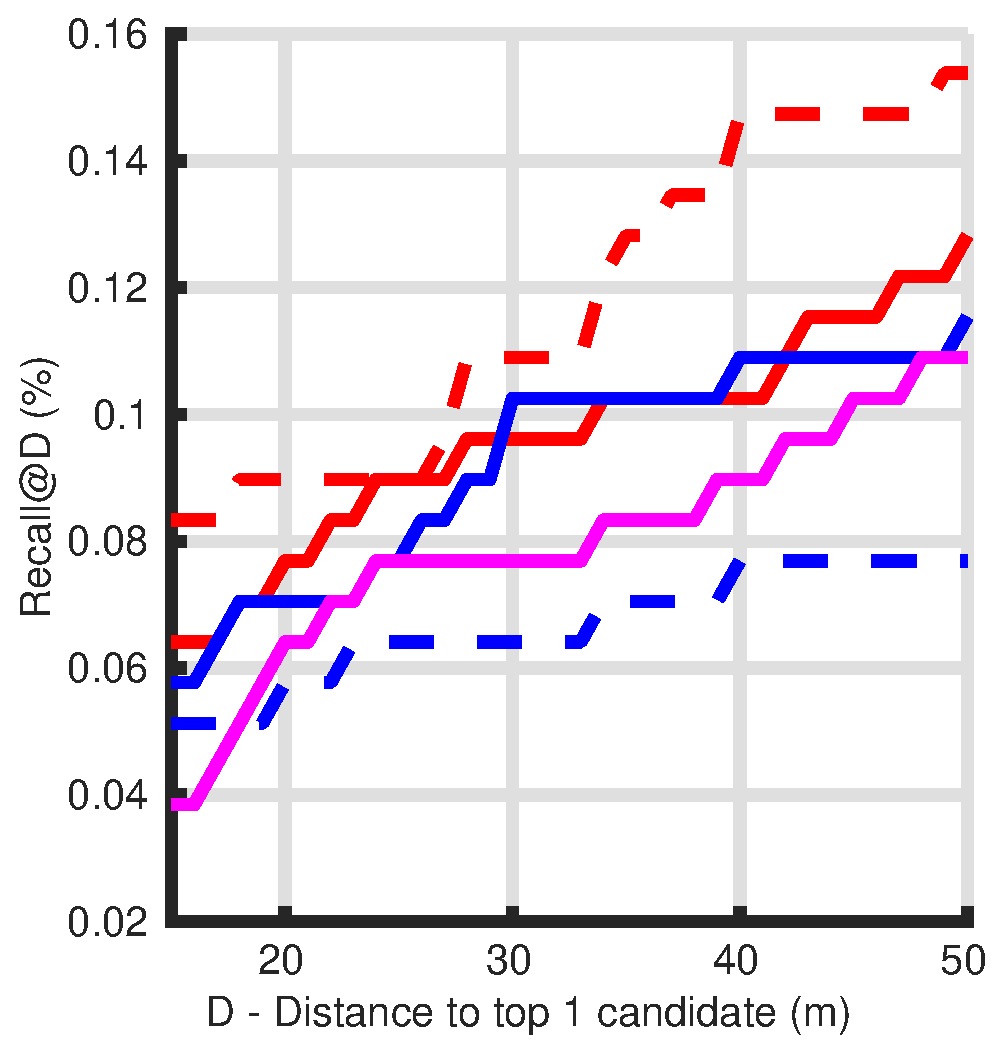
\includegraphics[width=\linewidth]{plot/oxf_cmu/Results_night_queries/distance}	
		
		\includegraphics[width=\linewidth]{plot/oxf_cmu/Results_night_queries/recall}
		
		c) Oxford -- Night
	\end{minipage}
	\begin{minipage}{0.16\linewidth}
		\center \scriptsize
		\includegraphics[width=\linewidth]{plot/oxf_cmu/Results_cmu_lt/distance}	
		
		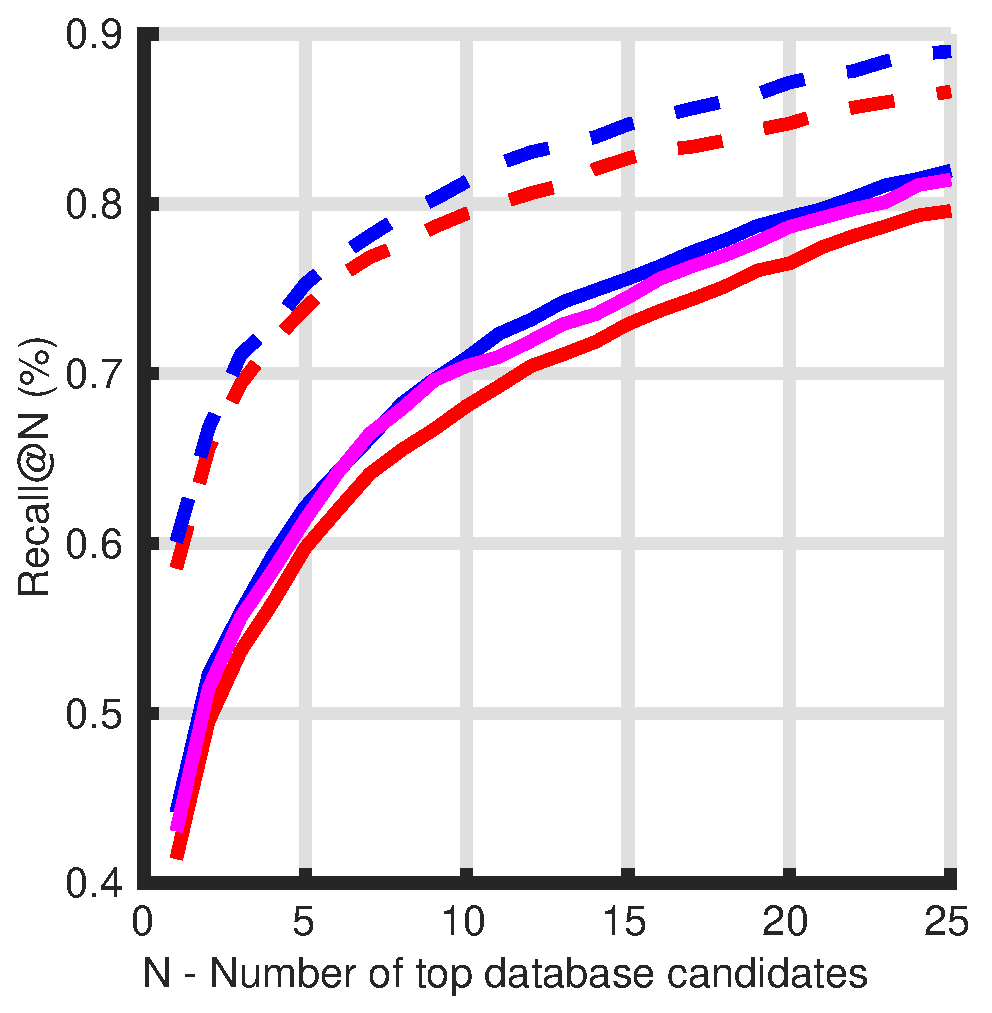
\includegraphics[width=\linewidth]{plot/oxf_cmu/Results_cmu_lt/recall}
		
		d) CMU -- LT
	\end{minipage}
	\begin{minipage}{0.16\linewidth}
		\center \scriptsize
		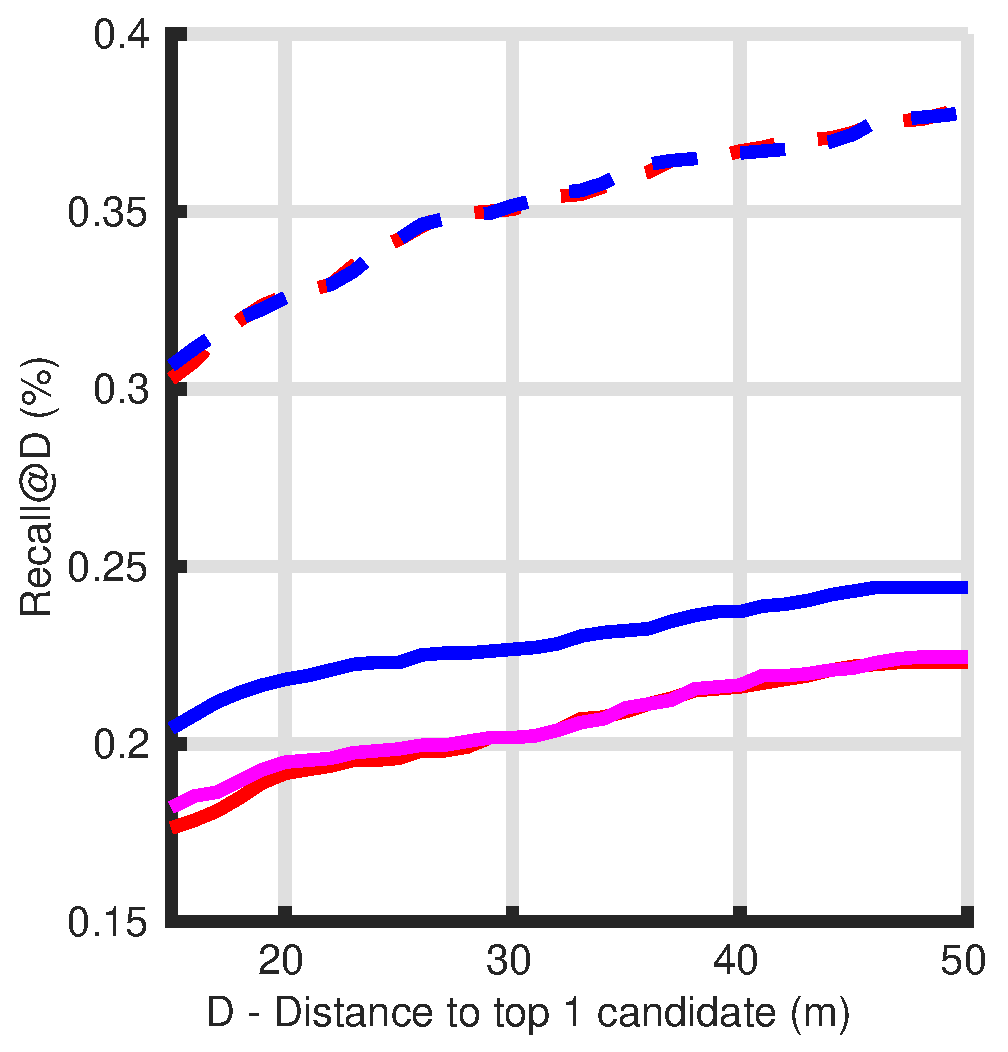
\includegraphics[width=\linewidth]{plot/oxf_cmu/Results_cmu_snow/distance}	
		
		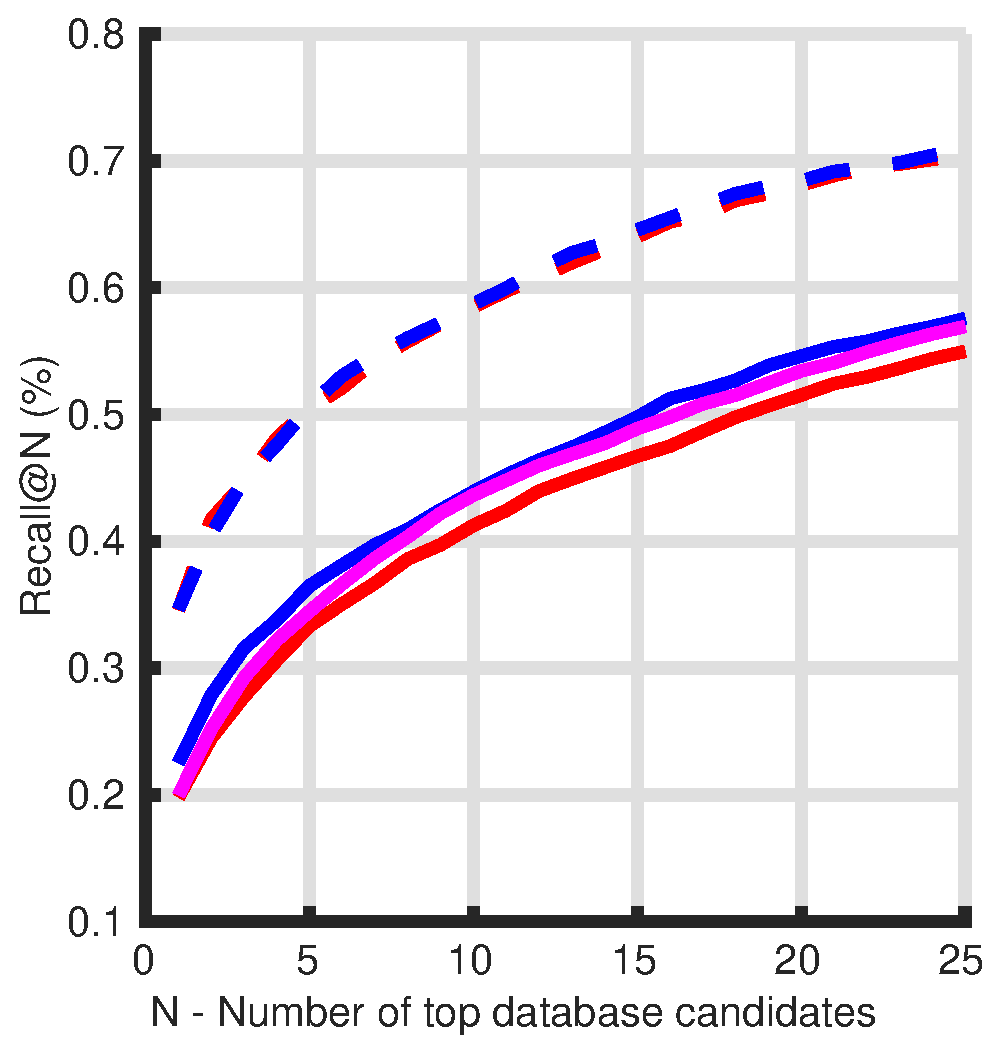
\includegraphics[width=\linewidth]{plot/oxf_cmu/Results_cmu_snow/recall}
		
		e) CMU -- Snow
	\end{minipage}
	\begin{minipage}{0.16\linewidth}
		\center \scriptsize
		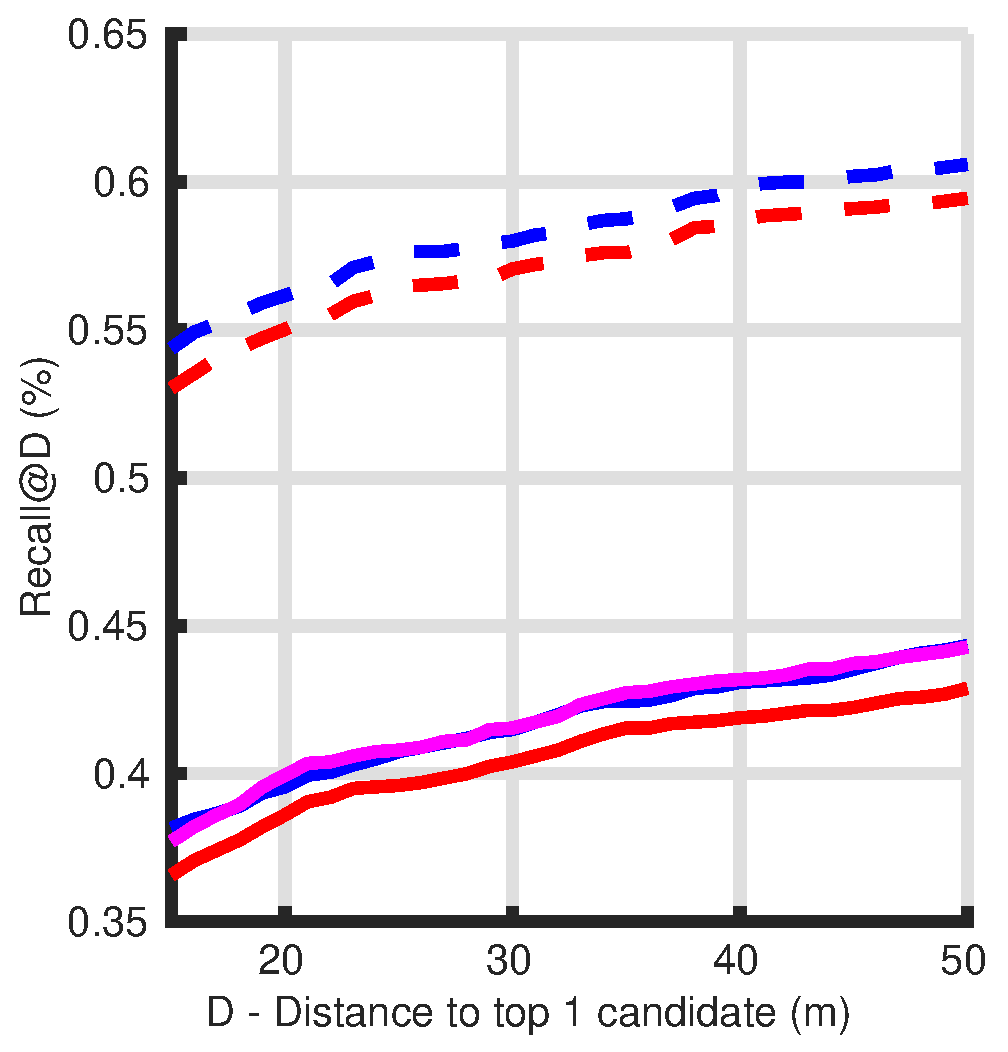
\includegraphics[width=\linewidth]{plot/oxf_cmu/Results_cmu_autumn/distance}	
		
		\includegraphics[width=\linewidth]{plot/oxf_cmu/Results_cmu_autumn/recall}
		
		f) CMU -- Autumn
	\end{minipage}
	
	\vspace{0.2cm}
	
	\begin{scriptsize}
	\begin{tabular}{c l c l c l c l c l }
		\textcolor{red}{\Large{--}} & Alexnet RGB & 
		\textcolor{red}{\Large{- -}} & Resnet RGB & 
		\textcolor{blue}{\Large{--}} & Alexnet RGB(D) (our) &
		\textcolor{blue}{\Large{- -}} & Resnet RGB(D) (our) &  
		\textcolor{magenta}{\Large{--}} & Alexnet RGB(H)  \\
	\end{tabular}		
	\end{scriptsize}
	
	\caption[Comparison of our method versus competitors]{\label{fig:results} \textbf{Comparison of our method RGB(D) versus hallucination network RGB(H) and networks trained with only images RGB}: we report results for backbone network encoder Resnet (- -) and Alexnet (--). Our method (\textcolor{blue}{in blue}) is superior in every scenario facing hallucination network (\textcolor{magenta}{in magenta}). It also beats, with a significant margin, networks trained with only images (\textcolor{red}{in red}). All the methods failed on the very challenging night to day scenario (b). Curves best viewed in colors.}
\end{figure}